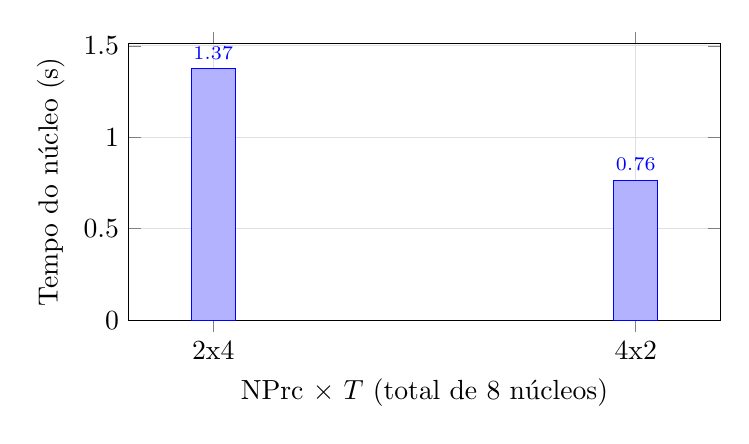
\begin{tikzpicture}
\begin{axis}[
    width=0.75\textwidth, height=0.42\textwidth,
    ybar, bar width=16pt, ymin=0,
    xlabel={NPrc $\times$ $T$ (total de 8 núcleos)}, ylabel={Tempo do núcleo (s)},
    symbolic x coords={2x4,4x2},
    xtick=data, enlarge x limits=0.2,
    nodes near coords, nodes near coords style={font=\scriptsize, /pgf/number format/.cd, fixed, precision=2},
    grid=major, grid style={gray!25},
]
\addplot coordinates {(2x4,1.374146) (4x2,0.763379)};
\end{axis}
\end{tikzpicture}
